\section{Vorläufige Zeitplanung}
gemäß den Leitfaden zur Durchführung von Bachelor-Abschlussarbeiten\cite{Boles:2015}, die Dauer der Bachelorarbeit beträgt vier Monate.\\
Der erste Teil der Zeit wird genutzt um das Projekt vollständig zu strukturieren. In der Einarbeitungsphase, wird das notwendige fehlende Wissen erworben.\\
Die dritte Phase befasst sich mit dem Entwurf der Softwareanwendung sowohl auf Datenbank- als auch auf Benutzeroberflächenebene sowie deren jeweiligen Tests.\\
In der Schreibphase, wird der Software-Quellcode wird dokumentiert, ein Benutzerhandbuch wird geschrieben und die schriftliche Ausarbeitung der Bachelorarbeit wird erstellt.
In der letzten Phase wird die Dokumentation vor der Abgabe überprüft und korrigiert, die Folien und Dokumente für den Vortrag werden geschrieben.

\begin{figure}[hp]%[H]
    \centering
    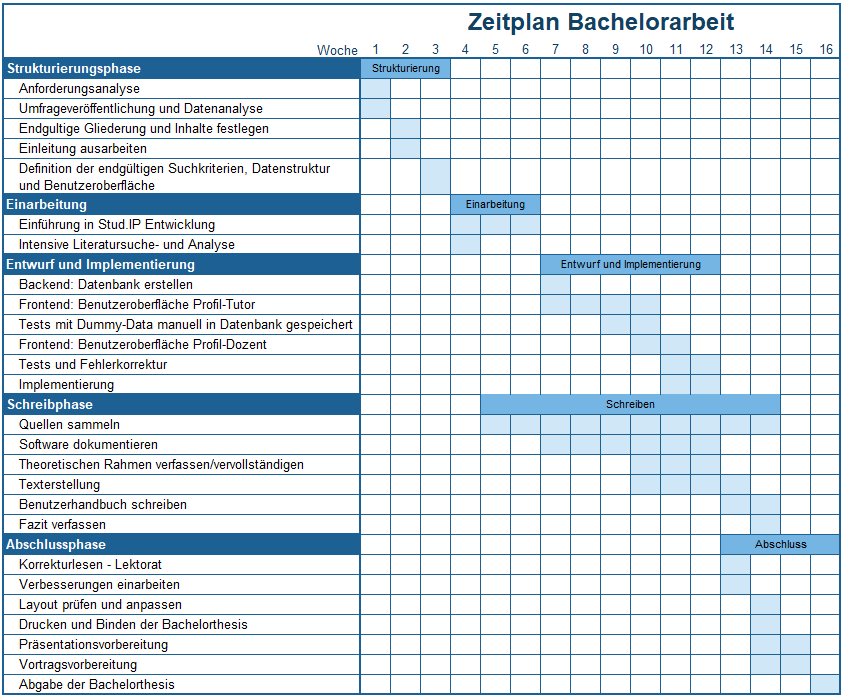
\includegraphics[height=12.5cm,keepaspectratio]{pics/zeitplan}\\
    \caption{Zeitplanung}
\end{figure}
